%%%%%%%%%%%%%%%%%%%%%%%%%%%%%%%%%%%%%%%%%%%%%%%%%%%%%%%%%%%%%%%%%%%%%%%%%%%%%%%
% Chapter 1 - Introduction
%%%%%%%%%%%%%%%%%%%%%%%%%%%%%%%%%%%%%%%%%%%%%%%%%%%%%%%%%%%%%%%%%%%%%%%%%%%%%%%

\chapter{Introduction} \label{ch:introduction}

Cerebrovascular diseases such as stroke are the fifth leading cause of death in the United States and the primary cause of chronic adult disability in the Western world \cite{Kochanek:ut}. Almost 800,000 people in the United States suffer a stroke each year with an estimated total medical cost of over \$40 billion \cite{Benjamin:2018gy}. Ischemic strokes represent approximately 87\% of all cases and occur when blood flow to the brain is disrupted by the formation of a thrombosis or embolism. While less prevalent, hemorrhagic strokes are associated with higher mortality rates \cite{Andersen:2009ih} and occur when an aneurysm or blood vessel ruptures in the brain. Patients who seek treatment within the first few hours of symptom onset have drastically improved outcomes compared to those who receive delayed care \cite{Hacke:2004kf}. The only FDA-approved pharmaceutical treatment for an ischemic stroke is recombinant tissue plasminogen activator (tPA), which enzymatically dissolves blood clots after being administered intravenously. However, only about 7\% of ischemic stroke patients ever receive the treatment, because it must be administered within the first three hours after the onset of symptoms \cite{Schwamm:2013bs}. Unless the patient qualifies for a catheter-based mechanical thrombectomy \cite{Smith:2008dd}, there are very few treatment options once the time window for tPA has passed. Chronic management relies upon pharmaceutical prophylaxis with anticoagulants, antihypertensives, and antihyperlipidemic statins, similar to that of other cardiovascular diseases \cite{StrokePreventioninAtrialFibrillationInvestigators:1991fl, TheStrokeCouncil:2004bi, Endres:2005bg}. Physical rehabilitation is often prescribed to help patients improve functional activity through residual neuroplasticity with varying degrees of efficacy \cite{Jette:2005ii, French:2010ka, Takeuchi:2013ce, French:2016hk}. Current research predominantly focuses on the development of new therapeutics targeting the circulatory and nervous systems through pharmacological, surgical, or behavioral interventions. These preclinical studies have a vital need for quantitative hemodynamic measurements to evaluate the efficacy of interventions in disease models of ischemic stroke.

Focal ischemic stroke is characterized by a localized reduction in blood flow to part of the brain following thrombotic or embolic occlusion of a blood vessel. The loss of blood supply rapidly triggers the ischemic cascade, a series of biochemical events that ultimately cause irreversible tissue damage and neuronal death \cite{Nesto:1987dx}. The region with the most severe reduction in blood flow is termed the ``ischemic core'' and can experience cellular death within minutes following the occlusion. Surrounding the core is the ``ischemic penumbra,'' a region of moderate to minimal ischemia supported by residual perfusion from collateral blood supply. Cellular death proceeds much more slowly in this metastable region as the infarct slowly expands into the penumbra over time \cite{Heiss:1992ge, Ginsberg:1999jy}. This has made the penumbra the primary target for neuroprotective interventions in an attempt to improve tissue viability and restrict the expansion of the core \cite{Felberg:2000gu, RamosCabrer:2011gz}. Understanding the hemodynamic mechanisms and metabolic burdens that affect the evolution of the ischemic penumbra is vital to improving the efficacy of stroke treatments.



%%%%%%%%%%%%%%%%%%%%%%%%%%%%%%%%%%%%%%%%%%%%%%%%%%%%%%%%%%%%%%%%%%%%%%%%%%%%%%%
% Section 1.1 - Imaging of Hemodynamics in the Brain
%%%%%%%%%%%%%%%%%%%%%%%%%%%%%%%%%%%%%%%%%%%%%%%%%%%%%%%%%%%%%%%%%%%%%%%%%%%%%%%
\section{Imaging of Hemodynamics in the Brain}

Modern medical imaging technology has revolutionized our ability to diagnose and treat pathologies in the human body. Many of these same techniques have also played a critical role in our fundamental understanding of the anatomy and physiology of the brain. Optical imaging modalities have been used extensively \cite{Hillman:2007ep} to study the hemodynamics of phenomena such as neurovascular coupling \cite{Liao:2013jl} and diseases such as stroke \cite{Obrig:2011hy}, epilepsy \cite{Bahar:2006es}, migraines \cite{Bolay:2002jg}, and Alzheimer's \cite{KoronyoHamaoui:2011hk}. However, optical imaging has limited clinical translation because of difficulties in delivering light through the thick, highly-scattering skull. Human hemodynamic studies typically rely upon well-established medical imaging technologies such as magnetic resonance imaging and positron-emission tomography.

%%%%%%%%%%%%%%%%%%%%%%%%%%%%%%%%%%%%%%%%%%%%%%%%%%%%%%%%%%%%%%%%%%%%%%%%%%%%%%%
\subsection{Non-Optical Methods}

The primary clinical technique for studying hemodynamic changes in the brain is magnetic resonance imaging (MRI) \cite{Calamante:2016dg}. MRI has the ability to observe both anatomical structure and localize functional dynamics without the need for exogenous contrast agents. Functional MRI (fMRI) depends upon blood-oxygen-level dependent (BOLD) contrast, which can detect relative changes in the concentration of deoxyhemoglobin, a strongly paramagnetic molecule \cite{Glover:2011eo}. The BOLD hemodynamic response reveals localized recruitment of oxygen via neurovascular coupling and gives fMRI the ability to measure the cerebral metabolic rate of oxygen consumption (\ce{CMRO2}), a metric correlated with brain activity. It also provides an indirect measure of cerebral blood flow (CBF) because \ce{CMRO2} is dependent upon regional blood flow. However, fMRI suffers from poor spatial and temporal resolutions, prohibiting it from examining neurovascular structure or hemodynamics in fine detail \cite{Glover:2011eo}.

Positron-emission tomography (PET) offers functional localization with high sensitivity at similar resolutions to fMRI but requires the injection or inhalation of a radioactive tracer \cite{Wintermark:2005dd}. CBF and \ce{CMRO2} can be measured using isotopes of oxygen gas or carbon dioxide while the cerebral metabolic rate of glucose consumption (CMRGlc), another proxy for brain activity, can be measured using \ce{^18F} fluorodeoxyglucose (FDG). PET requires access to cyclotron-produced radiopharmaceuticals and the instrumentation is rarely found outside of medical facilities. Radiation exposure also limits the number of successive imaging sessions that can be conducted in a subject.

Transcranial Doppler ultrasound offers measurements of CBF velocity in large arteries and veins and is an increasingly popular diagnostic and therapeutic monitoring tool \cite{Sarkar:2007fk}. Combined with anatomical information to obtain vessel size, the velocity measurements can be converted to volumetric flow. Clinically, the technique is limited to diagnosing global or hemispheric hypoperfusion because measurements are constrained to only the largest vessels \cite{Naqvi:2013hd}. However, the temporal resolution is significantly higher than fMRI or PET, which allows for dynamic monitoring of blood flow velocity over time.

%%%%%%%%%%%%%%%%%%%%%%%%%%%%%%%%%%%%%%%%%%%%%%%%%%%%%%%%%%%%%%%%%%%%%%%%%%%%%%%
\subsection{Optical Methods}

Optical imaging offers significantly higher spatial and temporal resolutions but with limited depth penetration compared to non-optical techniques. The increased resolution has facilitated the study of microscale brain hemodynamics and the complex relationship between neural activity and blood flow. However, spatial resolution is highly dependent upon gaining optical access to the area of interest, especially when imaging through highly-scattering tissues such as the skull. In animal models, the surgical implantation of optically-clear cranial windows is a common method to gain direct optical access to the surface of the brain.

Pulse oximetry to measure peripheral oxygen saturation (\ce{SO2}) is the most common clinical application of optical hemodynamic imaging. The non-invasive spectroscopic technique is based on absorption differences between oxygenated and deoxygenated hemoglobin and therefore requires no exogenous contrast agents. Transcranial near-infrared spectroscopy (NIRS) is a related technique that has been applied to visualizing functional \cite{Cui:2011en} and ischemic \cite{Murkin:2009eb} cerebral hemodynamics in humans. While it has limited clinical implementations \cite{Hoshi:2011gr}, results from NIRS have been strongly correlated with fMRI measurements in stroke patients \cite{Kato:2002ka}.

Hemoglobin has also been targeted as an endogenous contrast agent for optical intrinsic signal (OIS) imaging or multispectral reflectance imaging. These camera-based approaches measure changes in the reflectance of tissue at multiple wavelengths in order to estimate relative chromophore concentrations \cite{Zepeda:2004hc}. The resulting changes in oxy- and deoxyhemoglobin in response to stimuli are analogous to BOLD contrast from fMRI. OIS imaging has been performed during external stimulation to study the functional organization of the cortex at resolutions much greater than fMRI \cite{Tso:1990ba, Masino:1993tk}. Multispectral imaging has been combined with CBF estimates from laser speckle contrast imaging to measure the metabolic response to focal ischemia \cite{Jones:2008gb}.

Optical imaging can directly measure flow velocities within blood vessels by tracking or labeling erythrocytes. High frame rate cameras can be used for reflectance imaging of hemoglobin within cortical surface vasculature in order to follow erythrocyte motion \cite{Kazmi:2015du}. Alternatively, laser scanning microscopy of fluorescent contrast agents can be used to measure erythrocyte velocity within subsurface microvasculature \cite{Shih:2012bo}. Newer imaging techniques such as optical coherence tomography (OCT) now allow for cross-sectional, depth-resolved measurements of blood flow and hemoglobin concentrations \cite{Srinivasan:2009vx}.



%%%%%%%%%%%%%%%%%%%%%%%%%%%%%%%%%%%%%%%%%%%%%%%%%%%%%%%%%%%%%%%%%%%%%%%%%%%%%%%
% Section 1.2 - Measuring Blood Flow with Dynamic Light Scattering
%%%%%%%%%%%%%%%%%%%%%%%%%%%%%%%%%%%%%%%%%%%%%%%%%%%%%%%%%%%%%%%%%%%%%%%%%%%%%%%
\section{Measuring Blood Flow with Dynamic Light Scattering}

The monitoring of \textit{in vivo} blood flow dynamics is invaluable in both clinical and laboratory environments for understanding numerous physiological and pathophysiological phenomena. Angiographic techniques and ultrasound have garnered widespread adoption in clinics for providing anatomical and hemodynamic information. Optical imaging using dynamic light scattering (DLS) has become increasingly popular in preclinical research for measuring perfusion and has begun translating to clinical applications. The most common DLS techniques are laser Doppler flowmetry and laser speckle contrast imaging \cite{Briers:2001hy, Dunn:2011gi}. These two modalities are different strategies for imaging the same underlying physical phenomenon and are inherently based upon Doppler shifts in the frequency of coherent light caused by particle motion.

%%%%%%%%%%%%%%%%%%%%%%%%%%%%%%%%%%%%%%%%%%%%%%%%%%%%%%%%%%%%%%%%%%%%%%%%%%%%%%%
\subsection{Laser Doppler Flowmetry}

Laser Doppler flowmetry (LDF) relies upon the frequency spectrum analysis of backscattered coherent light to measure relative perfusion \cite{Briers:2001hy}. While it offers high temporal resolution, LDF is typically limited to measurements at a single spatial location. The introduction of scanning mirrors allow for spatially-resolved measurements at the expense of speed, with low-resolution (256 x 256 pixels) acquisitions taking several minutes in commercially available systems \cite{Rajan:2008di}. Full-field laser Doppler imaging (LDI) offers higher resolutions (480 x 480 pixels) at significantly faster speeds (14 frames per second) but relies upon expensive high frame rate cameras and complex acquisition hardware \cite{Lopez:2011bk}. LDF is frequently used as the ``gold standard'' during the development of newer DLS flowmetry techniques.

%%%%%%%%%%%%%%%%%%%%%%%%%%%%%%%%%%%%%%%%%%%%%%%%%%%%%%%%%%%%%%%%%%%%%%%%%%%%%%%
\subsection{Laser Speckle Contrast Imaging}

Laser speckle contrast imaging (LSCI) is a full-field optical imaging technique that provides instantaneous maps of blood flow by imaging time-varying laser speckle. The technique was first demonstrated by Fercher and Briers in 1981 using single-exposure photography of retinal blood flow \cite{Fercher:1981jh}. Because images were captured on film and required development prior to processing, the earliest LSCI instruments suffered from very low temporal resolutions and large uncertainties. The arrival of commercially available CCD cameras and faster computers in the 1990s allowed for near real-time LSCI perfusion measurements in the skin \cite{Briers:1995iu, Briers:1996kfa}. The technique was first applied to imaging CBF dynamics in rodents in 2001 \cite{Dunn:2001dj} and has since seen widespread adoption by the neuroscience community for animal studies on stroke \cite{Ayata:2004ba, Strong:2005kj, Armitage:2010ga}, spreading depression \cite{Ayata:2004ck, Shin:2006dc}, and functional activation \cite{Dunn:2005gw, Durduran:2016el}. LSCI has also seen clinical translation as an intraoperative tool for monitoring blood flow and perfusion during brain surgery \cite{Hecht:2009gu, Parthasarathy:2010gh}.

%%%%%%%%%%%%%%%%%%%%%%%%%%%%%%%%%%%%%%%%%%%%%%%%%%%%%%%%%%%%%%%%%%%%%%%%%%%%%%%
\subsubsection{Theory}

Laser speckle is the random interference pattern produced when coherent light scatters from a rough surface or inhomogeneous medium. It manifests because scattered photons travel slightly different path lengths, resulting in constructive and destructive interference between the out of phase coherent light waves. Imaging this scattered light produces a random two-dimensional interference pattern on the detector known as subjective speckle \cite{Ennos:1975et}. If the sample contains scattering particles in motion, such as erythrocytes flowing through vasculature, the speckle pattern will fluctuate temporally. Imaging a time-varying speckle pattern results in the integration of these temporal intensity fluctuations over the camera's exposure time. Assuming the exposure time is longer than the time scale of the speckle intensity fluctuations (\textless1 ms for biological tissues), the resulting speckle pattern will be blurred by the integration. Regions with greater motion will experience more rapid intensity fluctuations and therefore more blurring of the imaged speckle pattern. Because the dynamics of the speckle pattern encodes information about the underlying particle motion, a measure of flow can be obtained by quantifying the spatial blurring. This requires calculating the local speckle contrast ($K$), which is defined as the ratio between the standard deviation ($\sigma_s$) and the mean intensity of pixel values ($\langle{I}\rangle$) within a small region of the image at a single exposure time ($T$) \cite{Briers:1996kfa}.
%
% Equation - Speckle Contrast
\begin{equation}
    \label{eq:speckle_contrast}
    K(T) = \frac{\sigma_s(T)}{\langle{I}\rangle}
\end{equation}

A full speckle contrast image is obtained by computing Equation \ref{eq:speckle_contrast} within an $N$ x $N$ sliding window at every pixel of the raw image. The window size must be chosen carefully to ensure an accurate estimate of local contrast while maintaining adequate spatial resolution in the resulting image. Statistical analysis \cite{Duncan:2008hs} and past precedent \cite{Dunn:2011gi} have established $N = 7$ as an optimal window size and it is used exclusively throughout this dissertation. A properly sampled \cite{Kirkpatrick:2008ke} speckle pattern will produce speckle contrast values ranging between 0 and 1 \cite{Boas:2010vr}. When $K = 1$, there is no blurring of the speckle pattern and therefore no discernible motion in the sample during the camera exposure. However, when $K = 0$, the scattering particles are moving sufficiently fast to average out all the speckles.

% Figure - Simple LSCI Schematic
\begin{figure}
    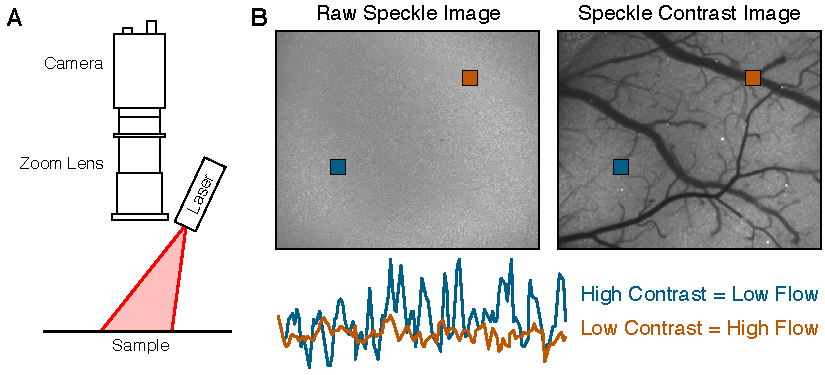
\includegraphics{figures/chapter_1/lsci_schematic.pdf}
    \caption{
        \label{fig:lsci_schematic}
        \textbf{(A)} Traditional LSCI microscope system consisting of an illuminating laser, imaging optics, and a camera. \textbf{(B)} Raw intensity image of the speckle pattern and the resulting speckle contrast image from vasculature in the mouse cerebral cortex. Regions of high contrast in the intensity image (blue) have low flow compared to regions with low contrast (orange), which have high flow.
    }
\end{figure}

An example of the raw intensity image of the speckle pattern and corresponding computed speckle contrast image are shown in Figure \ref{fig:lsci_schematic}B. The imagery was obtained \textit{in vivo} from the cerebral cortex of a mouse under general anesthesia. The graininess of the speckle pattern can be seen in the raw intensity image, with some regions appearing more blurred than others. The speckle contrast image was computed directly from the intensity image using Equation \ref{eq:speckle_contrast} to generate a two-dimensional map of motion for the field-of-view. Within the cortex, erythrocytes are the primary moving scattering particles and therefore vasculature is highlighted by the speckle contrast image. Regions of higher flow, such as a large vessel, experience more blurring of the speckle pattern and therefore have lower $K$ values. Conversely, regions of low flow, such as the space between resolvable surface vessels (parenchyma), experience less blurring and therefore have higher $K$ values. Measurements within the parenchyma sample the slower, more isotropic blood flow of unresolvable microvasculature beneath the surface of the cortex.

The shallow depth penetration of LSCI is a significant limitation of the imaging technique. Detected photons only sample a few hundred microns of superficial tissue without any depth resolution and are heavily-weighted towards large surface vasculature \cite{Davis:2014kc}. While skin and retinal imaging can be performed directly on the tissue of interest, CBF imaging requires either thinning or removing the skull to gain optical access \cite{Boas:2010vr}.

%%%%%%%%%%%%%%%%%%%%%%%%%%%%%%%%%%%%%%%%%%%%%%%%%%%%%%%%%%%%%%%%%%%%%%%%%%%%%%%
\subsubsection{Instrumentation}

The simple instrumentation necessary to perform LSCI has contributed to its popularity as a blood flow imaging technique. A basic LSCI microscope consists of an illuminating laser, imaging optics, and a camera (Figure \ref{fig:lsci_schematic}A). The laser output is expanded to broadly epi-illuminate the area of interest at a normal to oblique angle depending on the application. Red to near-infrared laser diodes (600-850 nm) are typically used to take advantage of the tissue optical window where scattering dominates absorption by hemoglobin or water. Because LSCI is based entirely upon scattering, wavelength is less important than other imaging techniques that rely upon absorption. However, the coherence length of the laser dictates the longest possible path length through the tissue that can be properly sampled for quantitative flow information. Lasers with narrow spectral bandwidths (e.g. single longitudinal mode or narrow linewidth lasers) offer coherence lengths of several meters and are more than sufficient for use in LSCI.

Camera selection varies broadly in literature and generally any charge-coupled device (CCD) or complementary metal-oxide-semiconductor (CMOS) camera is appropriate for use with LSCI \cite{Draijer:2008ic, Boas:2010vr}. Even cheap cameras such as webcams have been shown to provide reliable blood flow imagery \cite{Richards:2013bi}. While spectral sensitivity, bit depth, pixel size, frame rate, and noise are all important factors to consider, most researchers use the cameras readily available in their laboratory. However, it is critical that the speckle pattern is properly sampled such that the speckle size is at least twice the size of a single camera pixel \cite{Kirkpatrick:2008ke}. Deviation from the spatial Nyquist sampling criterion will reduce contrast and decrease the variation in the speckle contrast image.

%%%%%%%%%%%%%%%%%%%%%%%%%%%%%%%%%%%%%%%%%%%%%%%%%%%%%%%%%%%%%%%%%%%%%%%%%%%%%%%
\subsubsection{Quantitative Accuracy}

Speckle contrast values are only indicative of the amount of motion in a sample and are not linearly proportional to particle speed or volumetric flow. Understanding the nonlinear relationship with the complex underlying blood flow is an active area of research in the DLS field \cite{Duncan:2008fd, Briers:2013es}. Quantitative flow measurements require accurately relating the speckle contrast value to the characteristic decay time ($\tau_c$) of the speckle autocorrelation function. DLS theory has established that the speckle autocorrelation time is inversely proportional to the speed of the scatters in the single scattering regime \cite{Bonner:1981hga} and weighted by the number of dynamic scattering events under multiple scattering \cite{Boas:1997kf, Kazmi:2015du, Davis:2016ik}. Since Fercher and Briers first proposed a simple model relating $K$ and $\tau_c$ \cite{Fercher:1981jh}, there have been numerous improvements to more robustly extract the flow contributions from the observed speckle \cite{Bandyopadhyay:2005bg, Parthasarathy:2008el}. The model described by Bandyopadhyay \textit{et al.} \cite{Bandyopadhyay:2005bg} relates the measured $K$ with $\tau_c$:
%
% Equation - Bandyopadhyay Equation
\begin{equation}
    \label{eq:bandyopadhyay}
    K(T,\tau_c) = \left(\beta \frac{e^{-2x} - 1 + 2x}{2x^{2}}\right)^{1/2}
\end{equation}
%
where $x = T/\tau_c$, $T$ is the camera exposure time, and $\beta$ is a normalization factor that accounts for speckle averaging due to the mismatch between speckle size and pixel size, polarization, and the finite coherence length of the laser \cite{Lemieux:1999ko}. $\beta$ is frequently assumed to be equal to 1, limiting the technique to relative measures of flow. This model assumes that detected photons only experience single scattering interactions and that the underlying particle motion has a Lorentzian velocity distribution. Despite these assumptions, Equation \ref{eq:bandyopadhyay} has been used extensively to relate measured speckle contrast with relative blood flow \cite{Dunn:2011gi,Boas:2010vr} and will be used throughout this dissertation.

The inverse correlation time (ICT) is frequently interpreted as being proportional to the speed of the moving particles ($1/\tau_c \propto \nu_{scatterers}$) based on assumptions from laser Doppler flowmetry \cite{Bonner:1981hga}. While highly dependent upon the optical properties and flow conditions of the sample, ICT values in single vessels correspond to the speed of the flowing erythrocytes. In parenchyma regions, ICT is a measure of local perfusion because flow cannot be isolated to individual vessels from the depth integrated contributions of the unresolvable microvasculature \cite{Durduran:2016el, Dunn:2011gi}. Despite these assumptions and limitations, multiple studies have demonstrated strong correlations between LSCI estimates of CBF and absolute measurements from other perfusion indices \cite{Ayata:2004ba, Strong:2005kj, Kazmi:2015du}. The development of multi-exposure speckle imaging \cite{Parthasarathy:2008el} has improved the quantitative accuracy of the LSCI technique and will be discussed extensively in Chapter \ref{ch:mesi}.



%%%%%%%%%%%%%%%%%%%%%%%%%%%%%%%%%%%%%%%%%%%%%%%%%%%%%%%%%%%%%%%%%%%%%%%%%%%%%%%
% Section 1.3 - Measuring Oxygen Tension In Vivo
%%%%%%%%%%%%%%%%%%%%%%%%%%%%%%%%%%%%%%%%%%%%%%%%%%%%%%%%%%%%%%%%%%%%%%%%%%%%%%%
\section{Measuring Oxygen Tension \textit{In Vivo}}

\textit{In vivo} measurements of molecular oxygen have historically been made using highly invasive Clarke electrodes that are limited to point measurements outside the vascular lumen \cite{Vovenko:1999be, Tsai:2003cc, Roussakis:2015eu}. While targets as small as a few microns can be measured with the appropriate electrode, there are significant tradeoffs between the signal-to-noise ratio and spatial specificity depending on probe size. Electrodes can also only approximate intravascular oxygen concentrations through measurements in nearby interstitial tissue. Magnetic resonance techniques allow for noninvasive imaging of hemoglobin saturation, but suffer from low spatial resolutions and can only be correlated with free oxygen levels in the blood \cite{Roussakis:2015eu, Dunn:2003hg, Hou:2003hb, Liu:2006bt}. Oxygen-sensitive porphyrin probes allow for noninvasive, highly sensitive optical oxygenation measurements based on phosphorescence quenching \cite{Vinogradov:2012tda}. While an injection of the probe is required, absolute oxygen tension (\ce{pO2}) can be directly calculated from the lifetime of the measured phosphorescence decay.

%%%%%%%%%%%%%%%%%%%%%%%%%%%%%%%%%%%%%%%%%%%%%%%%%%%%%%%%%%%%%%%%%%%%%%%%%%%%%%%

\subsection{Oxygen-Dependent Quenching of Phosphorescence}
Recent advances in oxygen-sensitive probe design have made oxygen-dependent quenching of phosphorescence a powerful tool for \textit{in vivo} measurements of \ce{pO2} within both intravascular and interstitial spaces \cite{Vinogradov:2012tda, Esipova:2011hi}. This method relies upon dissolved environmental oxygen quenching the phosphorescence of porphyrin dyes or ruthenium complexes and causing a change in excited state lifetime (Figure \ref{fig:jablonski}A).  The \ce{pO2} can be quantified from the measured lifetime (Appendix \ref{app:stern_volmer}) using the Stern-Volmer relationship:
%
% Equation - Stern-Volmer Relationship
\begin{equation}
    \label{eq:stern-volmer}
    \frac{\tau_{0}}{\tau} = 1 + k_{q}\tau_{0}[pO_{2}]
\end{equation}
%
where $\tau$ is the measured phosphorescence lifetime, $\tau_{0}$ is the unquenched lifetime, and $k_{q}$ is a probe-specific quenching rate constant that depends upon the local environment (temperature, pH, atmospheric pressure, and salinity). Equation \ref{eq:stern-volmer} allows for the absolute \ce{pO2} to be obtained from the measured phosphorescence lifetime provided $k_q$ and $\tau_{0}$ are well-characterized under physiological conditions. Furthermore, because lifetime measurements are independent of absolute intensity, they can easily be isolated from other chromophores and tissue scattering, making them ideal for integration into multi-modal imaging systems.

% Figure - Jablonksi Diagram
\begin{figure}
    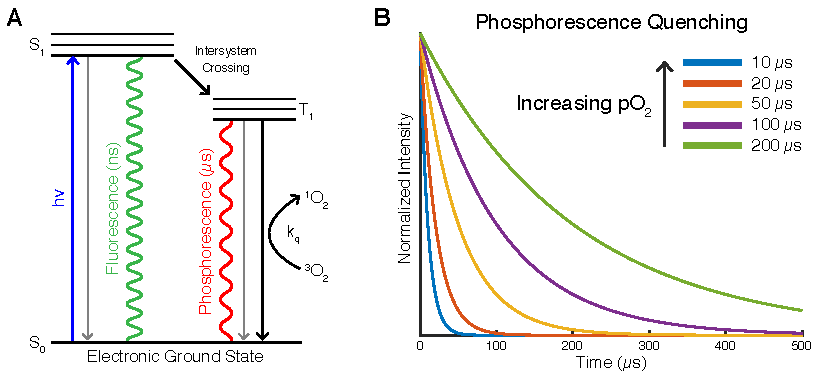
\includegraphics{figures/chapter_1/jablonski.pdf}
    \caption{
        \label{fig:jablonski}
        \textbf{(A)} Jablonski diagram of phosphorescence quenching by environmental molecular oxygen. \textbf{(B)} Phosphorescence quenching causes a reduction in the measured lifetime and is dependent upon [\ce{O2}] or \ce{pO2}.
    }
\end{figure}

The phosphorescence lifetime can be measured in the time domain by exciting the probe with a short pulse of light and collecting the emitted phosphorescence. The resulting phosphorescent decay curve can then be fit to an exponential to obtain the phosphorescence lifetime ($\tau$):
%
% Equation - Exponential Decay
\begin{equation}
    \label{eq:exponential_decay}
    I(t) = A + Be^{-t / \tau}
\end{equation}

Alternatively, frequency domain measurements can be made by calculating the phase shift or demodulation of the phosphorescence generated by sinusoidally-modulated light. While excitation light is utilized more efficiently in frequency domain measurements, they are more difficult to implement and process than time domain measurements.

Point detectors such as avalanche photodiodes or photomultiplier tubes are commonly used to acquire the phosphorescent decays because of their high sensitivity, gain, and temporal resolutions. However, these detectors limit the lifetime measurements to single spatial locations unless laser scanning systems \cite{Yaseen:2009ep, Kazmi:2013ey} or intensified exposure-gated cameras \cite{Shonat:2003ia, Sakadzic:2009jo} are utilized. Despite these limitations, \textit{in vivo} measurements of oxygen-dependent quenching of phosphorescence have been conducted in a variety of tissues including the retina, brain, muscle, and peritoneum \cite{Vovenko:1999be}. The technique has also been used extensively to study cortical oxygenation, often in conjunction with other imaging modalities \cite{Yu:2013fd, Devor:2014ke}.



%%%%%%%%%%%%%%%%%%%%%%%%%%%%%%%%%%%%%%%%%%%%%%%%%%%%%%%%%%%%%%%%%%%%%%%%%%%%%%%
% Section 1.4 - Research Overview
%%%%%%%%%%%%%%%%%%%%%%%%%%%%%%%%%%%%%%%%%%%%%%%%%%%%%%%%%%%%%%%%%%%%%%%%%%%%%%%
\section{Research Overview}

The overall goal of this project is the development of an optical imaging platform capable of the chronic monitoring of cortical hemodynamics during ischemic stroke and the subsequent recovery. The system combines two different imaging techniques, LSCI and oxygen-dependent quenching of phosphorescence, to measure CBF and \ce{pO2} within cortical vasculature. The development of the imaging system has four iterative milestones, each extending the capabilities of the platform. Chapter \ref{ch:system} details the initial design and construction of the dual-modality system and demonstrates acute \textit{in vivo} measurements in mice. Chapter \ref{ch:photothrombosis} describes modifications to the system to perform artery-targeted photothrombosis, an update to the conventional photothrombotic model of ischemic stroke. The technique is demonstrated \textit{in vivo} with the acute and chronic hemodynamics monitored using the imaging platform. The functional effects of the targeted infarct on fine motor skills are also examined. Chapter \ref{ch:mesi} details the implementation of multi-exposure speckle imaging to improve the robustness of chronic CBF measurements. Finally, Chapter \ref{ch:awake} describes the transition to awake animal imaging and demonstrates chronic imaging of the recovery from targeted photothrombotic stroke.



%%%%%%%%%%%%%%%%%%%%%%%%%%%%%%%%%%%%%%%%%%%%%%%%%%%%%%%%%%%%%%%%%%%%%%%%%%%%%%%
% END Chapter 1
%%%%%%%%%%%%%%%%%%%%%%%%%%%%%%%%%%%%%%%%%%%%%%%%%%%%%%%%%%%%%%%%%%%%%%%%%%%%%%%
